% PAKETE UND DOKUMENTKONFIGURATION
\documentclass[11pt, a4paper]{article}

% Encoding für Umlaute
\usepackage[utf8]{inputenc}
\usepackage[T1]{fontenc}

% Silbentrennung
\usepackage[ngerman]{babel}

% erweiterte Matheumgebungen und Formelnummer mit Sectionnummer
\usepackage{amsmath}
\numberwithin{equation}{section}

% Braket Notation
\usepackage{braket}
\usepackage{isotope}
\usepackage{mhchem}

% zusätzliche mathematische Schriftarten
\usepackage{amsfonts}

% verschiedene mathematische Symbole
\usepackage{amssymb}

% Einheiten setzen z.B. \SI{10}{\kilo\gram\meter\per\second\squared}
% Fehler: \SI{10 +- 0,2e-4}{\metre}
\usepackage{siunitx}
\sisetup{
  output-decimal-marker={,},
  separate-uncertainty
}

% Einheitendefinitionen
\DeclareSIUnit{\skt}{Skt.}
\DeclareSIUnit{\gauss}{G}

% Operatordefinitionen
\DeclareMathOperator{\erf}{erf}

% Randbreiten
\usepackage[left=3.5cm,right=3.5cm,top=3cm,bottom=3cm,twoside]{geometry}

% Bilder einfügen
\usepackage{graphicx}

% Verweise innerhalb des Dokuments
\usepackage{hyperref}
\hypersetup{
	colorlinks = true,
	allcolors = {black}
}

% bessere Tabellenlayouts
\usepackage{booktabs}
\usepackage{multirow}
\usepackage{multicol}

% Seitenlayout (Kopfzeile)
\usepackage{fancyhdr}

% Float Barriers
\usepackage{placeins}

% Pakete für gedrehte Subfigures
\usepackage{caption}
\usepackage{subcaption}
\usepackage{rotating}

% Paket für textumflossene Abbildungen und Tabellen
\usepackage{wrapfig}

\usepackage{float}

% Caption-Setup
\captionsetup{font={small}}
\renewcommand{\thefigure}{\thesection.\arabic{figure}}
\renewcommand{\thesubfigure}{\alph{subfigure}}
\renewcommand{\thetable}{\thesection.\arabic{table}}
\renewcommand{\thesubtable}{\alph{subtable}}

% Manuelle Silbentrennung
\hyphenation{Re-so-na-tor Mo-den-ab-stand Re-so-na-tor-län-ge Spek-t-ro-me-ter}

% Tiefe des Inhaltsverzeichnisses (Level: 1 sections, 2 subsections,
% 3 subsubsections)
\setcounter{tocdepth}{3}

% FANCYHDR SETUP
\pagestyle{fancy}
\fancyhead[EL,OR]{\thepage}
\fancyhead[ER]{\leftmark}
\fancyhead[OL]{\rightmark}

\renewcommand{\sectionmark}[1]{
\markboth{\thesection{} #1}{\thesection{} #1}
}
\renewcommand{\subsectionmark}[1]{
\markright{\thesubsection{} #1}
}

% DOKUMENTINFORMATIONEN
\title{P521 \\ Gamma-Spektroskopie mit Szintillations- und Halbleiterdetektoren}

\author{Christopher Deutsch\footnote{christopher.deutsch@uni-bonn.de} \and Christian Bespin\footnote{christian.bespin@uni-bonn.de}}

\date{\today}

\begin{document}

\begin{titlepage}

\maketitle

% DURCHFÜHRUNGSDATUM UND TUTOR
\begin{center}
\begin{tabular}{l r}
Durchführung: & 07./08. April 2015 \\
Gruppe: & $\alpha$ 6 \\
Tutor: & Yannick Wunderlich
\end{tabular}
\end{center}

% ZUSAMMENFASSUNG
\begin{abstract}
\noindent

\end{abstract}

\end{titlepage}

% INHALTSVERZEICHNIS
\tableofcontents
% Neue Seite nach TOC
\newpage

% INHALT VERSUCHSPROTOKOLL

\section{Einführung}

\section{Theorie}

\subsection{Radioaktiver Zerfall}

\subsubsection{Quellen radioaktiver Strahlung}
\label{sssec:quellen_radioaktivität}
Man kategorisiert Quellen radioaktiver Strahlung meistens in \textbf{natürliche Radioaktivität} und \textbf{künstliche Radioaktivität}.
Zu ersterem werden vor allem radioaktive Nuklide gezählt, die bereits seit Entstehung der Erde existieren und heute noch nachweisbar sind (primordiale Nuklide).
Weiterhin werden Nuklide, die bei Zerfällen dieser entstehen sowie kosmische Strahlung der natürlichen Radioaktivität zugeordnet.
Künstliche Radioakivität entsteht gezielt oder als Abfallprodukt bei gesteuerten Prozessen wie der Kernspaltung zur Energiegewinnung oder für medizinischen und technischen Anwendungen.

\subsubsection{Zerfallsreihen}

Als Zerfallsreihe bezeichnet man eine Kette radioaktiver Zerfälle, bei denen das aus dem zerfallenden Nuklid entstehende Tochternuklid weiter über radioaktiven Zerfall zerfällt.
Von besonderem Interesse sind die natürlichen Zerfallsreihen, die diese Kette radioaktiver Zerfälle für die primordialen Nuklide (s. \ref{sssec:quellen_radioaktivität}) beschreiben.
Es werden hier nur einige der Nuklide aufgeführt, da die Reihen recht lang sind und sich zwischendurch auch verzweigen können (dies geschieht, wenn ein Nuklid in mehrere andere zerfallen kann).
\begin{align*}
	&\isotope[244]{Pu}\to\dots\to\isotope[232]{Th}\to\dots\to\isotope[228]{Th}\to\dots\to\isotope[208]{Pb} &\qquad\text{(Thoriumreihe)}\\
	&\isotope[238]{U}\to\dots\to\isotope[226]{Ra}\to\dots\to\isotope[214]{Pb}\to\dots\to\isotope[206]{Pb} &\qquad\text{(Uran-Radium-Reihe)}\\
	&\isotope[235]{U}\to\dots\to\isotope[227]{Ac}\to\dots\to\isotope[211]{Pb}\to\dots\to\isotope[207]{Pb} &\qquad\text{(Uran-Actinium-Reihe)}
\end{align*}
Die als Thoriumreihe bezeichnete Zerfallsreihe beginnt zwar mit einem Pulloniumnuklid, ist jedoch nach dem am häufigsten auftretenden Element Thorium benannt.
Es existiert darüber hinaus noch eine Neptunium-Reihe ($\isotope[237]{Np}\to\isotope[205]{Tl}$), diese zählt aber nicht mehr zu den natürlichen Zerfallsreihen, da das bei Entstehung der Erde Neptunium vorhandene Neptunium mittlerweile komplett zerfallen ist.
Sie kann nur noch auf künstlichem Weg erzeugt werden, da \isotope[237]{Np} ein Tochternuklid von in Kernreaktoren erzeugten Nukliden ist.


\subsubsection{$\gamma$-Strahlung}

\subsection{Wechselwirkung von $\gamma$-Quanten mit Materie}

\subsubsection{Photoeffekt}
Absorption eines Photons durch ein atomisches Elektron
\begin{align*}
	E_\mathrm{e^{-}} = h \nu - E_\mathrm{Bind.}
\end{align*}
Nur im Atom, da der Kern den Rückstoß absorbieren muss (Impulserhaltung).
\begin{align*}
	\sigma_\mathrm{Photo.} \propto
	\begin{cases}
		Z^5 E_\gamma^{-\frac{7}{2}} & E_\gamma < m_\mathrm{e} c^2 \\
		Z^5 E_\gamma^{-1} & E_\gamma > m_\mathrm{e} c^2
	\end{cases}
\end{align*}
Quelle: Siegbahn
\begin{figure}[h]
	\centering
	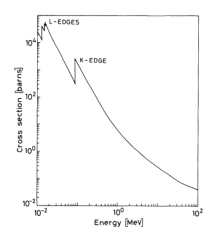
\includegraphics{./figures/photoeffekt.png}
	\caption{Photoeffekt Blei: William R. Leo}
	\label{fig:photoeffekt}
\end{figure}

\subsubsection{Compton-Effekt}
Streuung von Photonen an freien Elektron.
In Materie wenn $E_\gamma \gg E_\mathrm{Bind. e^{-}}$ dann Elektronen effektiv frei.

(BILD mit Winkeln undso)

\begin{align}
	\frac{E_\gamma^\prime}{E_\gamma} &= \frac{1}{1 + \frac{h \nu}{m_\mathrm{e} c^2} (1-\cos\theta)} \\
	\Delta \lambda &= \lambda_\mathrm{c} (1 - \cos\theta) \\
	\lambda_\mathrm{c} &= \frac{h}{m_\mathrm{e} c}
\end{align}
Wirkungsquerschnitt gegeben durch Klein-Nishina:
\begin{align}
	\sigma_\mathrm{c} \propto \frac{Z}{E_\gamma}
\end{align}

Compton-Kante...

Kein Energietransfer:\\
Thomson-Streuung: Compton im klassischen Limit\\
Rayleigh-Streuung: Streuung am ganzen Atom\\


\subsubsection{Paarbildung}
\begin{align}
	\gamma \rightarrow \mathrm{e}^{+} + \mathrm{e}^{-}\\
	E_\gamma \geq 2 m_\mathrm{e} c^2
\end{align}

\begin{align}
	\sigma_\mathrm{Paar} \propto Z^2 \ln E_\gamma
\end{align}

\subsubsection{Summe aller Effekte}

Bildah

\subsection{Szintillatoren, Halbleiterdetektor, Photomulti etc.}

\subsection{Spektrum, Vielkanalanalysator}

\subsection{Auflösungsvermögen, Breite, Unterschiede der Detektoren}

\subsection{Nachweiswahrscheinlichkeit}

\subsection{Termschemata}


\section{Versuchsaufbau}

\section{Durchführung und Auswertung}
Die ausführliche Durchführung ist der Versuchsanleitung \cite{anleitung} zu entnehmen.
Sollten Abweichungen bei der Durchführung auftreten, so werden diese im jeweiligen Unterkapitel dargestellt.

\section{Fazit}

\FloatBarrier
% BIBLIOGRAPHIE
\vspace{\fill}
% Maximale Anzahl der Einträge in Klammer
% Zitieren mit \cite{lamport94}
\begin{thebibliography}{19}

\bibitem{krane}
	Kenneth S. Krane,
	\emph{Introductory Nuclear Physics},
	John Wiley \& Sons 1988

\bibitem{mayer-kuckuk}
	Theo Mayer-Kuckuk,
	\emph{Kernphysik - Eine Einführung} (7. Auflage),
	Teubner 2002

\bibitem{siegbahn}
	K. Siegbahn,
	\emph{Alpha-, Beta- and Gamma-Ray Spectroscopy},
	Elsevier Science Ltd. 1965

\bibitem{hillert}
	W. Hillert,
	\emph{physics612: Accelerator Physics},
	Universität Bonn 2014

\bibitem{anleitung}
	Physikalisches Praktikum V: Kern- und Teilchenphysik,
	Versuchsbeschreibung \emph{P523: $\beta$-Spektrometer} (Stand: Januar 2015),
	Universität Bonn	

\bibitem{fermi_function}
	Venkataramaiah, P.; Gopala, K.; Basavaraju, A.; Suryanarayana, S.S.; Sanjeevia, H.
	\emph{A simple relation for the Fermi function},
	Journal of Physics G 11 (3): 359-364

\bibitem{riezler}
	Riezler, W.; Kopitzki, K.
	\emph{Kernphysikalisches Praktikum},
	Teubner 1963

\bibitem{tl_literatur}
  C.J. Chiara, F.G. Kondev,
  Nuclear Data Sheets 111,141 (2010),
  \url{http://www.nndc.bnl.gov/nudat2/decaysearchdirect.jsp?nuc=204TL&unc=nds}
  (Letzter Aufruf: 16. April 2015)

\bibitem{na_literatur}
  R.B. Firestone,
  Nuclear Data Sheets 106, 1 (2005)
  \url{http://www.nndc.bnl.gov/nudat2/decaysearchdirect.jsp?nuc=22NA&unc=nds}
  (Letzter Aufruf: 16. April 2015) 

\end{thebibliography}

% APPENDIX
\begin{appendix}
\section{Anhang}
Auf den folgenden Seiten sind der Vollständigkeit halber alle gemessenen Werte sowie die jeweils zur Auswertung berechneten Werte zusammengetragen.
\clearpage

\end{appendix}

\end{document}
